\documentclass[letterpaper,10pt]{article}

\usepackage{listings}
\usepackage{color}
\usepackage{tikz}

\setlength{\headheight}{0in}
\setlength{\marginparsep}{0in}
\setlength{\footskip}{0in}
\setlength{\headsep}{0in}
\setlength{\marginparwidth}{0in}
\setlength{\marginparpush}{0in}
\setlength{\voffset}{0in}
\setlength{\hoffset}{-1in}
\setlength{\voffset}{-1in}
\setlength{\oddsidemargin}{0.75in}
\setlength{\evensidemargin}{0.75in}
\setlength{\topmargin}{0.75in}
\setlength{\textheight}{9.5in}
\setlength{\textwidth}{7in}
\setlength{\parindent}{0in}
\setlength{\parskip}{10pt} %change this to match font size

\pagestyle{empty}
\definecolor{gray}{gray}{0.75}
\usetikzlibrary{shapes,arrows,calc}
\lstset{numbers=left,backgroundcolor=\color{gray},frame=single}

% define block styles
\tikzstyle{line} = [draw, -latex']
\tikzstyle{block} = [draw, rectangle, text centered, minimum height=2em]
\tikzstyle{mlblock} = [draw, rectangle, text width=10em, text centered, minimum height=2em]
\tikzstyle{decision} = [draw, diamond, text width=4.5em, text centered, node distance=3cm, inner sep=0pt]
\tikzstyle{cloud} = [draw, rectangle, text centered, rounded corners, minimum height=2em]

\begin{document}
    Albert Chang and Nipun Chopra\\
    CSE-380 A6\\
    University at Buffalo\\
    Dr. Kris Schindler\\
    February 17, 2011\\
    \textit{Lab 3 Documentation}

    The objective of Lab 3 was to write five subroutines, named
    \textit{read\_string}, \textit{output\_string}, \textit{mod},
    \textit{uart\_init}, and \textit{lab3}. Ultimately, the goal of all
    subroutines created a program that provided the modulo of two numbers
    provided by the user. It would give immediate feedback by displaying what
    the user input through the serial. The range of numbers was also limited
    between 0 and 99,999.

    The majority of the lab was already done through previous lab objectives.
    The \textit{mod} routine required only one line to be changed in the
    \textit{division} routine from lab 2, so that it returned the remainder
    instead of the quotient. The \textit{read\_character} and
    \textit{output\_character} routines were made in the first part of this lab.
    And finally, the \textit{uart\_init} routine was a simple rewrite of the
    \textit{serial\_init} function from the C wrapper that was provided. The
    only codes that needed to be split up between the two were the
    \textit{read\_string} and \textit{output\_string} routines.

    Although it would've been more efficient for subroutines to perform checks,
    it was decided that  the checks would be placed in the main \textit{lab3}
    routine. This would ensure the subroutines keep to their functions, never
    leaving the scope of the job they were to perform. What we gain is the
    routines are more portable. The other routines can be used by any other
    routines. If we wanted to reuse these pieces of code, the custom checks may
    need to be changed or remove completely to be compatible.
    
    The trade-off for this added portability is there are added branching
    instructions and there are added instructions for constructing and
    destructing strings for analysis.

    The flow of the main routine appears linear in the flowchart. However,
    there are some loops to acomplish the conversion of a string to an
    integer and a string into an integer.

    In order to convert a string to an integer, we iterate through the string,
    converting each digit from the ascii value to the integer it represents.
    As we iterate, to combine the other digits, multiply the current integer
    by 10, and add the next one.

    Converting from integer to string needed a little more work. The lowest
    digit is extracted by moduloing the number by 10, and divide by 10.

    \begin{center}
    \begin{tikzpicture}[node distance=1.5cm, auto]
        \node[cloud] (origin) {Start};
        \node[block, below of=origin] (uart) {Initialize UART0};
        \node[block, below of=uart] (interrupt) {Initialize interrupts};
        \node[block, below of=interrupt] (speed) {Setup initial speed};
        \node[block, below of=speed] (output) {Initial output};
        \node[block, below of=output] (time) {Start timer};
        \node[cloud, below of=time] (stop) {Stop};
        \path[line] (origin) -- (uart);
        \path[line] (uart) -- (interrupt);
        \path[line] (interrupt) -- (speed);
        \path[line] (speed) -- (output);
        \path[line] (output) -- (time);
        \path[line] (time) -- (stop);
    \end{tikzpicture}
\end{center}


    The \textit{division} flowchart was simply copied over from Lab 2 to use
    for the \textit{mod} flowchart. Note that although the flowchart is
    unchanged, there was a line that was changed so that it returned the
    remainder instead of the quotient. An additional return was added on
    to help with converting a string to integer.

    \begin{center}
    \begin{tikzpicture}[node distance = 1.5cm, auto]
        \node[cloud] (origin) {Start};
        \node[block, below of=origin] (initq) {Initialize Quotient to 0};
        \node[block, below of=initq] (initr) {Initialize Remainder};
        \node[block, below of=initr] (initc) {Initialize Counter to 16};
        \node[block, below of=initc] (lsldivor) {Logical Shift Left Divisor 16 Places};
        \node[block, below of=lsldivor] (subr) {Remainder := Remainder - Divisor};
        \node[decision, below of=subr] (rcheck) {Is\\Remainder $<$ 0 ?};
        \node[block, right of=rcheck, node distance = 7cm] (addr) {Remainder := Remainder + Divisor};
        \node[mlblock, below of=addr] (lsq0) {Logical Shift Quotient\\LSB = 0};
        \node[mlblock, below of=rcheck, node distance = 3cm] (lsq1) {Logical Shift Quotient\\LSB = 1};
        \node[mlblock, below of=lsq1] (msb) {Right Shift Divisor\\MSB=0};
        \node[decision, below of=msb] (ccheck) {Is Counter $\leq$ 1 ?};
        \node[block, left of=ccheck, node distance = 5cm] (dcount) {Decrement Counter};
        \node[cloud, below of=ccheck, node distance = 3cm] (stop) {Stop};
        \path[line] (origin) -- (initq);
        \path[line] (initq) -- (initr);
        \path[line] (initr) -- (initc);
        \path[line] (initc) -- (lsldivor);
        \path[line] (lsldivor) -- (subr);
        \path[line] (subr) -- (rcheck);
        \path[line] (rcheck) -- node [near start] {yes} (addr);
        \path[line] (addr) -- (lsq0);
        \path[line] (rcheck) -- node [near start] {no} (lsq1);
        \path[line] (lsq0) |- (msb);
        \path[line] (lsq1) -- (msb);
        \path[line] (msb) -- (ccheck);
        \path[line] (ccheck) -- node [near start] {yes} (dcount);
        \path[line] (dcount) |- (subr);
        \path[line] (ccheck) -- node [near start] {no} (stop);
    \end{tikzpicture}
\end{center}


    The \textit{read\_character} flowchart came from lecture.

    \begin{center}
    \begin{tikzpicture}[node distance = 1.5cm, auto]
        \node[cloud] (origin) {Start};
        \node[decision, below of=origin] (test) {Test RDR in status register};
        \node[block, below of=test, node distance = 3.5cm] (read) {Read byte from receive register};
        \node[cloud, below of=read] (stop) {Stop};
        \path[line] (origin) -- (test);
        \path[line] (test) -- node [near start] {1} (read);
        \path[line] (test) -| node [near start] {0} +(3,2) -- +(0,2);
        \path[line] (read) -- (stop);
    \end{tikzpicture}
\end{center}


    The \textit{output\_character} flowchart also came from lecture.

    \begin{center}
    \begin{tikzpicture}[node distance = 1.5cm, auto]
        \node[cloud] (origin) {Start};
        \node[decision, below of=origin] (test) {Test THRE in status register};
        \node[block, below of=test, node distance = 3.5cm] (store) {Store byte in transmit register};
        \node[cloud, below of=store] (stop) {Stop};
        \path[line] (origin) -- (test);
        \path[line] (test) -- node [near start] {1} (store);
        \path[line] (test) -| node [near start] {0} +(3,2.25) -- +(0,2.25);
        \path[line] (store) -- (stop);
    \end{tikzpicture}
\end{center}


    The \textit{uart\_init} routine was a simple linear routine.
    \begin{center}
    \begin{tikzpicture}[node distance = 3cm, auto]
        \node[cloud] (origin) {Start};
        \node[block, below of=origin, node distance=1.5cm] (enable) {Write 0x5 to PINSEL0 to enable UART0};
        \node[mlblock, below of=enable] (init) {Configure U0LCR:\\%
                                                8-bit word length\\%
                                                1 stop bit\\%
                                                no parity\\%
                                                disable break control\\%
                                                enable access latch};
        \node[block, below of=init] (baud) {Set baud rate to 9600};
        \node[mlblock, below of=baud] (conf) {Configure U0LCR:\\%
                                                8-bit word length\\%
                                                1 stop bit\\%
                                                no parity\\%
                                                disable break control\\%
                                                disable latch access};
        \node[cloud, below of=conf] (stop) {Stop};
        \path[line] (origin) -- (enable);
        \path[line] (enable) -- (init);
        \path[line] (init) -- (baud);
        \path[line] (baud) -- (conf);
        \path[line] (conf) -- (stop);
    \end{tikzpicture}
\end{center}


    mod\_ui\_wrapper.c
    \lstinputlisting[language=C]{../mod_ui_wrapper.c}

    mod\_ui.s
    \lstinputlisting{../mod_ui.s}

\end{document}
